\documentclass[12pt]{article}

\title{Activity 11: Designing Classes}
\author{Chris Mayfield and Helen Hu}
\date{July 2017}

%\ProvidesPackage{cspogil}

% fonts
\usepackage[utf8]{inputenc}
\usepackage[T1]{fontenc}
\usepackage{mathpazo}

% spacing
\usepackage[margin=2cm]{geometry}
\renewcommand{\arraystretch}{1.4}
\setlength{\parindent}{0pt}

% orphans and widows
\clubpenalty=10000
\widowpenalty=10000
\pagestyle{empty}

% figures and tables
\usepackage{graphicx}
\usepackage{multicol}
\usepackage{tabularx}
\usepackage{wrapfig}

% fixed-width columns
\usepackage{array}
\newcolumntype{L}[1]{>{\raggedright\let\newline\\\arraybackslash\hspace{0pt}}m{#1}}
\newcolumntype{C}[1]{>{\centering\let\newline\\\arraybackslash\hspace{0pt}}m{#1}}
\newcolumntype{R}[1]{>{\raggedleft\let\newline\\\arraybackslash\hspace{0pt}}m{#1}}

% include paths
\makeatletter
\def\input@path{{Models/}{../../Models/}}
\graphicspath{{Models/}{../../Models/}}
\makeatother

% colors
\usepackage[svgnames,table]{xcolor}
\definecolor{bgcolor}{HTML}{FAFAFA}
\definecolor{comment}{HTML}{007C00}
\definecolor{keyword}{HTML}{0000FF}
\definecolor{strings}{HTML}{B20000}

% table headers
\newcommand{\tr}{\bf\cellcolor{Yellow!10}}

% syntax highlighting
\usepackage{textcomp}
\usepackage{listings}
\lstset{
    basicstyle=\ttfamily\color{black},
    backgroundcolor=\color{bgcolor},
    numberstyle=\scriptsize\color{comment},
    commentstyle=\color{comment},
    keywordstyle=\color{keyword},
    stringstyle=\color{strings},
    columns=fullflexible,
    keepspaces=true,
    showlines=true,
    showstringspaces=false,
    upquote=true
}

% code environments
\newcommand{\java}[1]{\lstinline[language=java]{#1}}%[
\lstnewenvironment{javalst}{\lstset{language=java,backgroundcolor=}}{}
\lstnewenvironment{javabox}{\lstset{language=java,frame=single,numbers=left}\quote}{\endquote}

% PDF properties
\usepackage[pdftex]{hyperref}
\urlstyle{same}
\makeatletter
\hypersetup{
  pdftitle={\@title},
  pdfauthor={\@author},
  pdfsubject={\@date},
  pdfkeywords={},
  bookmarksopen=false,
  colorlinks=true,
  citecolor=black,
  filecolor=black,
  linkcolor=black,
  urlcolor=blue
}
\makeatother

% titles
\makeatletter
\renewcommand{\maketitle}{\begin{center}\LARGE\@title\end{center}}
\makeatother

% boxes [optional height]
\newcommand{\emptybox}[1][10em]{
\vspace{1em}
\begin{tabularx}{\linewidth}{|X|}
\hline\\[#1]\hline
\end{tabularx}}

% models
\newcommand{\model}[1]{\section{#1}\nopagebreak}
\renewcommand{\thesection}{Model~\arabic{section}}

% questions
\newcommand{\quest}[1]{\subsection*{Questions~ (#1)}}
\newcounter{question}
\newcommand{\Q}{\vspace{1em}\refstepcounter{question}\arabic{question}.~ }
\renewcommand{\thequestion}{\#\arabic{question}}

% sub-question lists
\usepackage{enumitem}
\setenumerate[1]{label=\alph*)}
\setlist{itemsep=1em,after=\vspace{1ex}}

% inline answers
\definecolor{answers}{HTML}{C0C0C0}
\newcommand{\ans}[1]{%
\ifdefined\Student
    \leavevmode\phantom{~~\textcolor{answers}{#1}}
\else
    ~~\textcolor{answers}{#1}
\fi}

% longer answers [optional height]
\newsavebox{\ansbox}
\newenvironment{answer}[1][4em]{
\nopagebreak
\begin{lrbox}{\ansbox}
\begin{minipage}[t][#1]{\linewidth}
\color{answers}
}{
\end{minipage}
\end{lrbox}
\ifdefined\Student
    \phantom{\usebox{\ansbox}}%
\else
    \usebox{\ansbox}%
\fi}


\begin{document}

\maketitle

Previously we explored how classes define attributes and methods.
Static variables and methods apply to the whole class, whereas non-static variables and methods apply to specific objects.
%In this activity, we'll take a closer look at what objects look like.

\guide{
  \item Discuss benefits of POGIL for student learning.
  \item Explain the purpose of constructor, accessor, and mutator methods.
  \item Implement the equals and toString methods for a given class design.
  \item Design a new class (UML diagram) based on a general description.
}{
  \item Identifying key attributes and data types that model a real-world object. (Problem Solving)
}{
TODO

Ask the managers to pace their team on Model 1; they will need to work quickly. Set aside 10 minutes between Models 1 and 2 to step through Circle.java using \href{http://pythontutor.com/java.html}{Java Tutor} or similar tool. Have the recorder document team misconceptions on his/her activity sheet.

When reporting out Model 2, have presenters write their designs on whiteboards. Compare the trade-offs of different designs: to store credit card numbers, some teams may use strings, others arrays, some int/long.
}

%TODO add new model for equals and toString
% based on Model 2 of "Activity 10 - Class Design" by Helen Hu

\model{Class Design}

Classes are often used to represent abstract data types, such as \java{Color} or \java{Point}.
They are also used to represent objects in the real world, such as \java{CreditCard} (see next page) or \java{Person}.
%UML class diagrams summarize the attributes and methods of a class.

\begin{center}
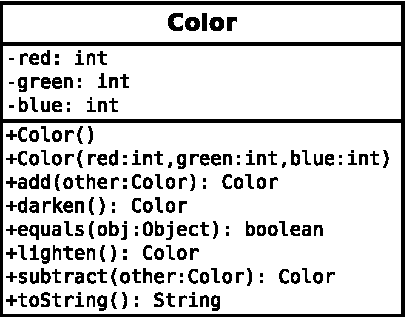
\includegraphics{Color.pdf}  % immutable
~~~~~
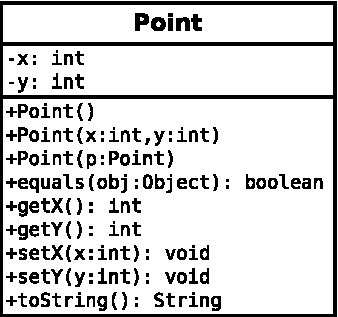
\includegraphics{Point.pdf}  % mutable
\end{center}

Classes generally include the following kinds of methods (in addition to others):
\begin{itemize}[itemsep=0pt]
\item \textbf{constructor} methods that initialize new objects
\item \textbf{accessor} methods (getters) that return attributes
\item \textbf{mutator} methods (setters) that modify attributes
\item \textbf{object} methods such as \java{equals} and \java{toString}
%\item \textbf{utility} methods which are generally static
\end{itemize}


\quest{20 min}


\Q Identify the constructors for the \java{Color} class. What is the difference between them? What arguments do they take?

\begin{answer}
There are two constructors: one that takes three integers for the RGB values, and other that takes a Color object. The latter is called a \emph{copy constructor}. Constructors do not return values.
\end{answer}


\Q Identify an accessor method in the \java{Point} class. 
\begin{enumerate}[itemsep=1pt]
\item Which instance variable does it get? \ans{{\tt this.x} or {\tt this.y}}
\item What arguments does the method take? \ans{none}
\item What does the method return? \ans{The value of \java{x} or \java{y}}
\end{enumerate}


\Q Identify a mutator method in the \java{Point} class.
\begin{enumerate}[itemsep=1pt]
\item Which instance variable does it set? \ans{{\tt this.x} or {\tt this.y}}
\item What arguments does the method take? \ans{The value of \java{x} or \java{y}}
\item What does the method return? \ans{nothing}
\end{enumerate}


\begin{center}
\textit{For the remaining questions, you will design a class that represents an individual's credit card.}
\bigskip\par
% https://www.bankofamerica.com/credit-cards/

\includegraphics{credit-card.png}
\end{center}


\Q List two or more attributes that would be necessary for this \java{CreditCard} class. For each attribute, indicate what data type would be most appropriate.

\begin{answer}[5em]
Answers may include \verb|number:long|, \verb|expire:Date|, \verb|name:String|, \verb|code:int|, etc.
\end{answer}


\Q When constructing (or updating) a \java{CreditCard} object, what values would you need to check? What are the valid ranges of values for each attribute?

\begin{answer}[5em]
The number should have 16 digits, dates need to have valid months and days, names should be at most 22 letters and not contain digits or other characters, code should be 3--4 digits.
\end{answer}


\Q List two accessor methods would be appropriate for the \java{CreditCard} class.
Include arguments and return values, using the same format as a UML diagram.

\begin{answer}[5em]
\begin{verbatim}
+getNumber(): long
+getExpire(): Date
+getName(): String
+getCode(): int
\end{verbatim}
\end{answer}


\Q List two mutator methods would be appropriate for the \java{CreditCard} class.
Include arguments and return values, using the same format as a UML diagram.

\begin{answer}[5em]
\begin{verbatim}
+setNumber(number:long): void
+setExpire(expire:Date): void
+setName(name:String): void
+setCode(code:int): void
\end{verbatim}
\end{answer}

%TODO add new meta activity: POGIL Research

\end{document}
